\documentclass[aspectratio=169]{beamer}

\usetheme{Madrid}
\usecolortheme{DSLAB}
\usefonttheme[onlylarge]{structurebold}
\setbeamerfont*{frametitle}{size=\normalsize,series=\bfseries}
\setbeamertemplate{navigation symbols}{}

\usepackage[utf8]{inputenc} 
\usepackage[T1]{fontenc}
\usepackage[english]{babel}
\usepackage{xmpmulti}
\usepackage{tikz}
\usepackage{pgf}
\usepackage{amsmath}
\usepackage{amsfonts}
\usepackage{graphicx}
\usepackage{color}
\usepackage{multirow}
\usepackage{lmodern}
\usepackage{hyperref}
\usepackage{eurosym}
\usepackage{listings}
\usepackage{booktabs}

\lstset{
  basicstyle=\ttfamily\small,
  frame=single,
  breaklines=true,
  showstringspaces=false,
  columns=fullflexible
}


\usetikzlibrary{arrows}
\tikzstyle{block}=[draw opacity=0.7,line width=1.4cm]

\setbeamercovered{dynamic}
\setbeamerfont{author}{family=\rmfamily}
\institute[URJC]{DSLAB}

\author[Big Data Processing II]{
	Alberto Fernández Isabel \\
	Natalia Madrueño Sierro \\
	Rubén Rodríguez Fernández \\
}

\title[Presentación]{
	Big Data Processing II \\ \vspace{0.2em}
	IA Generativa aplicada al deporte \\ \vspace{0.2em}
    Retrieval-Augmented Generation (RAG)
}
\date{Marzo 2026}
\titlegraphic{
\includegraphics[width=3cm]{images/logos/logourjceps.png}}


\setbeamertemplate{section page}{
	\vspace{1cm}
	\begin{beamercolorbox}[sep=8pt,center,wd=\textwidth]{section title}
		\usebeamerfont{section title}\insertsection\par 
	\end{beamercolorbox}
}


% =====================================================
\begin{document}

\begin{frame}
\titlepage
\end{frame}

%------------------------------------------------
\section{Mapa del bloque}
\frame{\sectionpage}

\begin{frame}{Arquitectura conceptual del bloque}
\begin{center}
\Large
\begin{tabular}{c}
{\color{gray2}\textbf{Sesión 1}} \\ 
{\color{gray2}Control del comportamiento} \\
{\color{gray2}\small Prompt Engineering + Post-training}
\\[0.1em]
$\Downarrow$
\\[0.1em]
{\color{colorblue}\textbf{Sesión 2}} \\ 
{\color{colorblue}Control de la información} \\
{\color{colorblue}\small Retrieval-Augmented Generation (RAG)}
\\[0.1em]
$\Downarrow$
\\[0.1em]
{\color{gray2}\textbf{Sesión 3}} \\ 
{\color{gray2}Control del flujo y la acción} \\
{\color{gray2}\small Agentes, Tools y Arquitecturas Cognitivas}
\end{tabular}
\end{center}
\end{frame}

% =====================================================
\section{Introducción}
\frame{\sectionpage}

\begin{frame}{El límite epistemológico del LLM}

Un LLM modela una distribución condicional:

\[
P(y \mid x)
\]

donde:
\begin{itemize}
    \item $x$ = prompt + contexto disponible
    \item $y$ = secuencia generada
\end{itemize}

\vspace{0.4em}

Pero:
\begin{itemize}
    \item No tiene acceso directo a bases de datos externas.
    \item No consulta sistemas internos.
    \item No distingue entre dato real y patrón aprendido.
\end{itemize}

\textbf{Conclusión:} conocimiento aprendido $\neq$ acceso a información actualizada.

\end{frame}

% -----------------------------------------------------

\begin{frame}{Por qué el Prompting no resuelve esto}
\begin{columns}[T]
\column{0.5\textwidth}

El Prompt Engineering:

\begin{itemize}
    \item Controla estructura.
    \item Reduce ambigüedad.
    \item Define formato.
\end{itemize}

Pero:

\[
Prompting \not\Rightarrow Acceso\ a\ datos\ externos
\]

\vspace{0.4em}

\textbf{No modifica la base informacional del modelo}.

\column{0.5\textwidth}
\centering
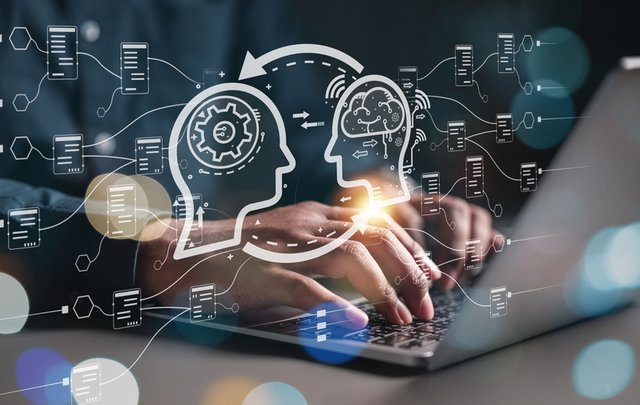
\includegraphics[width=0.9\textwidth]{images/presentacion/intro.jpg}
\end{columns}

\end{frame}

% -----------------------------------------------------

\begin{frame}{El problema en Ciencia de Datos Deportivos}

Un sistema real dispone de:

\begin{itemize}
    \item Tracking físico por partido.
    \item Métricas avanzadas (xG, PPDA, presiones).
    \item Informes médicos.
    \item Observaciones de scouting.
\end{itemize}

Pregunta crítica:

\begin{quote}
¿Ha disminuido la intensidad de presión tras acumular más de 300 minutos en 10 días?
\end{quote}

\textbf{Un LLM aislado no puede responder correctamente.}

\end{frame}

% =====================================================
\section{Definición de RAG}
\frame{\sectionpage}

\begin{frame}{Definición operacional de RAG}

Retrieval-Augmented Generation introduce un mecanismo externo:

\[
Output = f(Prompt + Retrieve(Query))
\]

\begin{itemize}
    \item Retrieve(Query) devuelve fragmentos relevantes.
    \item El LLM genera condicionado por ese contexto.
\end{itemize}

\vspace{0.4em}

No cambia parámetros del modelo.  
Cambia la evidencia disponible en inferencia.

\end{frame}

% -----------------------------------------------------

\begin{frame}{Separación conceptual del sistema}

\begin{columns}[T]
\column{0.5\textwidth}
\begin{tabular}{ll}
\toprule
\textbf{Componente} & \textbf{Rol} \\
\midrule
Embeddings & Representación semántica \\
Vector DB & Indexación eficiente \\
Retriever & Selección de contexto \\
LLM & Síntesis condicionada \\
\bottomrule
\end{tabular}

\vspace{0.5em}

RAG es una arquitectura distribuida, no una simple extensión del modelo.

\column{0.5\textwidth}
\centering
 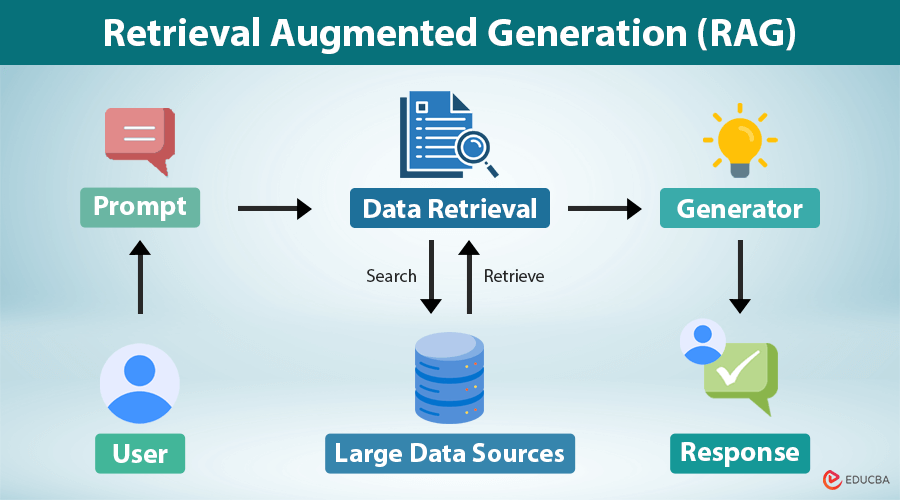
\includegraphics[width=0.9\textwidth]{images/presentacion/rag.png}
\end{columns}
\end{frame}

% =====================================================
\section{Diseño técnico de RAG}
\frame{\sectionpage}

\begin{frame}{Chunking: decisión crítica}

\begin{columns}[T]
\column{0.5\textwidth}
Dividir documentos implica:

\begin{itemize}
    \item Elegir \textbf{tamaño de fragmento}.
    \item Definir \textbf{solapamiento}.
    \item Preservar \textbf{coherencia semántica}.
\end{itemize}

Errores comunes:

\begin{itemize}
    \item Chunk demasiado grande → baja precisión.
    \item Chunk demasiado pequeño → pérdida de contexto.
    \item Solapamiento excesivo → redundancia y coste.
\end{itemize}

\column{0.5\textwidth}
\centering
 \vspace{5em}
 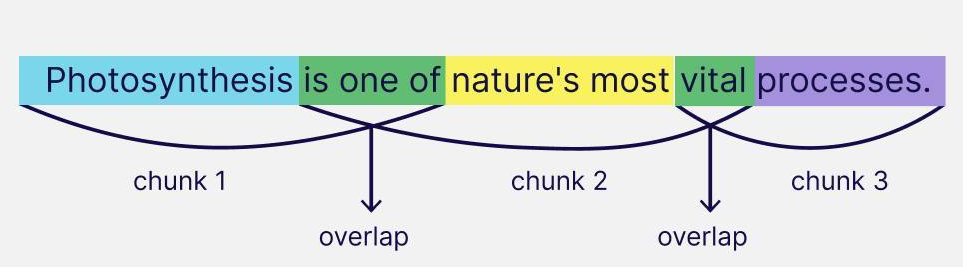
\includegraphics[width=0.9\textwidth]{images/presentacion/chunking.png}
\end{columns}

\end{frame}

% -----------------------------------------------------

\begin{frame}{Embeddings: representación semántica}

Un embedding es una función:

\[
E : Texto \rightarrow \mathbb{R}^d
\]

Permite medir similitud semántica.

Limitaciones:

\begin{itemize}
    \item No captura bien relaciones numéricas exactas.
    \item Puede perder contexto temporal.
    \item Similaridad $\neq$ relevancia estadística.
\end{itemize}

\end{frame}

% -----------------------------------------------------

\begin{frame}{Búsqueda por similitud}
\begin{columns}[T]
\column{0.5\textwidth}
Similitud típica:

\[
sim(u,v) = \frac{u \cdot v}{\|u\|\|v\|}
\]

Pero:

\begin{itemize}
    \item Similaridad semántica no garantiza pertinencia.
    \item Sensible a redacción del query.
\end{itemize}

La calidad del retrieval es crítica.
\column{0.5\textwidth}
\centering
 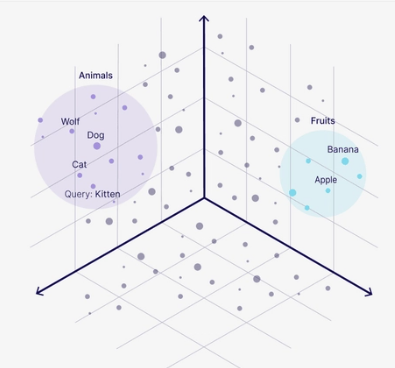
\includegraphics[width=0.9\textwidth]{images/presentacion/vectors.png}
\end{columns}
\end{frame}

% -----------------------------------------------------

\begin{frame}{Vector Database y metadatos en fútbol}
\begin{columns}[T]
\column{0.5\textwidth}
Un sistema robusto debe permitir:

\begin{itemize}
    \item Filtrado por temporada, jugador, competición.
    \item Indexación por tipo de documento.
    \item Actualización incremental.
\end{itemize}

Sin metadatos, el retrieval pierde precisión contextual.

\column{0.5\textwidth}
\centering
 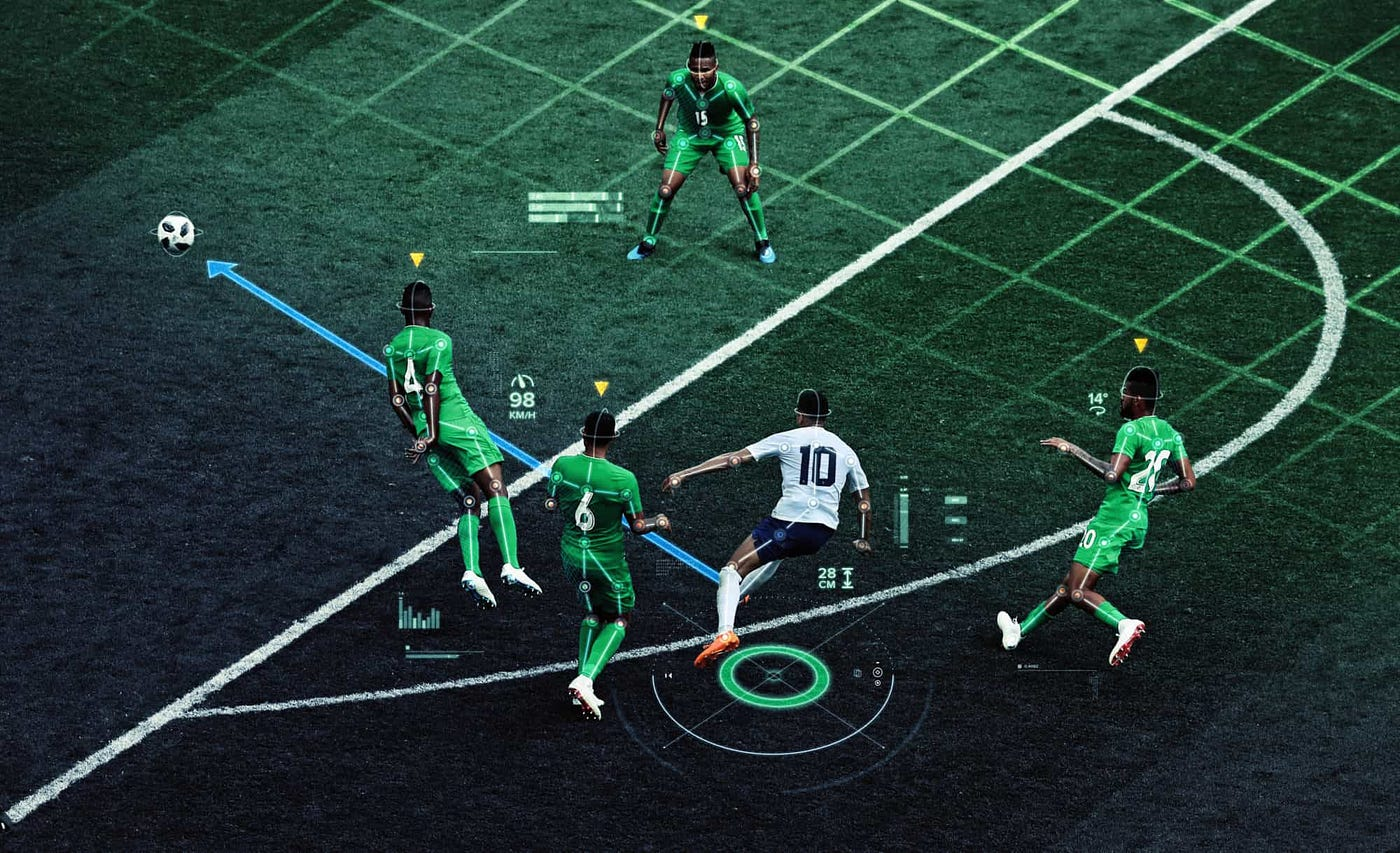
\includegraphics[width=0.9\textwidth]{images/presentacion/futbol.jpg}
\end{columns}
\end{frame}

% =====================================================
\section{Pipeline completo}

\begin{frame}{Pipeline detallado}

Cada etapa introduce posible error. \\
\centering
\begin{tikzpicture}[
    node distance=1.2cm,
    every node/.style={font=\small},
    process/.style={
        rectangle,
        rounded corners,
        draw=colorblue,
        fill=colorblue!15,
        align=center,
        minimum width=4.0cm,
        minimum height=0.9cm
    },
    arrow/.style={->, thick}
]

\node (q) [process] {Query del usuario};
\node (emb) [process, below of=q] {Embedding del query};
\node (ret) [process, below of=emb] {Retrieval Top-$k$};
\node (ctx) [process, below of=ret] {Construcción del contexto};
\node (gen) [process, below of=ctx] {Generación con LLM};
\node (post) [process, below of=gen] {Postprocesamiento};

\draw [arrow] (q) -- (emb);
\draw [arrow] (emb) -- (ret);
\draw [arrow] (ret) -- (ctx);
\draw [arrow] (ctx) -- (gen);
\draw [arrow] (gen) -- (post);

\end{tikzpicture}

\end{frame}

% -----------------------------------------------------

\begin{frame}{Trade-off fundamental}
\begin{columns}[T]
\column{0.5\textwidth}
\[
Veracidad \uparrow \Rightarrow Coste \uparrow
\]

\begin{itemize}
    \item Más contexto → más tokens.
    \item Más tokens → mayor latencia.
    \item Mayor latencia → menor escalabilidad.
\end{itemize}

Diseñar \textbf{RAG es optimizar} este equilibrio.
\column{0.5\textwidth}
\centering
 
\includegraphics[width=0.9\textwidth]{images/presentacion/tradeoff.png}
\end{columns}
\end{frame}

% =====================================================
\section{Aplicaciones en deporte}
\frame{\sectionpage}

\begin{frame}{RAG sobre métricas históricas}
\begin{columns}[T]
\column{0.5\textwidth}
Base interna:

\begin{itemize}
    \item Métricas por partido.
    \item Indicadores avanzados.
    \item Carga física acumulada.
\end{itemize}

Consulta:

\begin{quote}
Compara evolución de presión alta con descanso < 72h.
\end{quote}

Requiere filtrado + recuperación + síntesis.

\column{0.5\textwidth}
\centering
 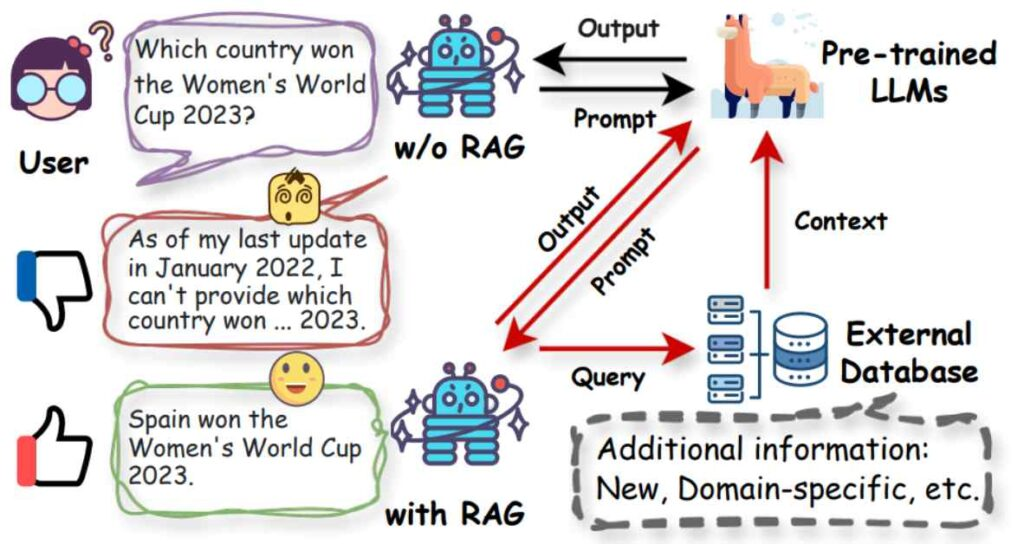
\includegraphics[width=0.9\textwidth]{images/presentacion/rag2.jpg}
\end{columns}

\end{frame}

% -----------------------------------------------------

\begin{frame}{RAG sobre scouting textual}
\begin{columns}[T]
\column{0.5\textwidth}
Documentos:

\begin{itemize}
    \item Informes técnicos.
    \item Observaciones cualitativas.
\end{itemize}

Permite:

\begin{itemize}
    \item Búsqueda semántica.
    \item Detección de patrones recurrentes.
    \item Síntesis multi-documento.
\end{itemize}

\column{0.5\textwidth}
\centering
 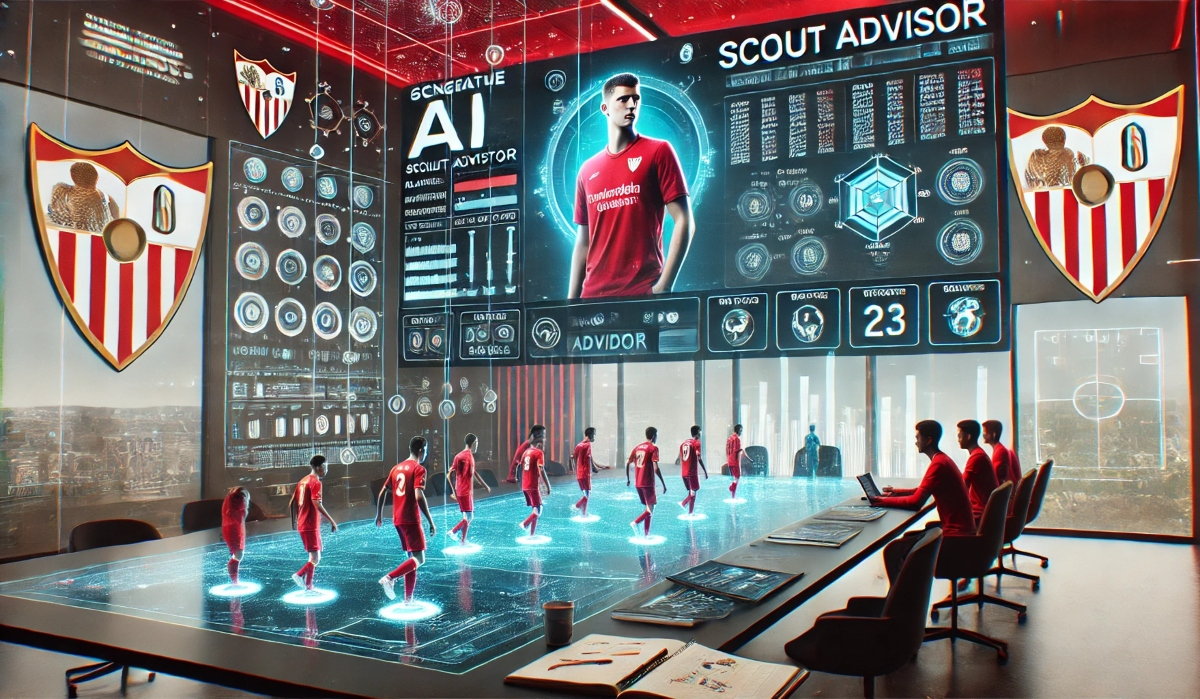
\includegraphics[width=0.9\textwidth]{images/presentacion/sevilla.jpg}
\end{columns}

\end{frame}

% -----------------------------------------------------

\begin{frame}{RAG híbrido: texto + cálculo}

\textbf{Problema}:

Embeddings no gestionan bien números exactos.

Solución:

\begin{itemize}
    \item \textbf{Recuperación textual} (búsqueda semántica en RAG).
    \item \textbf{Cálculo determinista externo} (fórmulas programadas).
    \item \textbf{Inyección de resultados estructurados} (creación de tablas numéricas).
\end{itemize}

Arquitectura híbrida = mayor precisión.

\end{frame}

% =====================================================
\section{Limitaciones}
\frame{\sectionpage}

\begin{frame}{Error compuesto}
\begin{columns}[T]
\column{0.5\textwidth}
RAG introduce dos fuentes de error:

\[
Error_{total} = Error_{retrieval} + Error_{generation}
\]

\textbf{Un mal retrieval no se compensa con mejor modelo}.

\column{0.5\textwidth}
\centering
 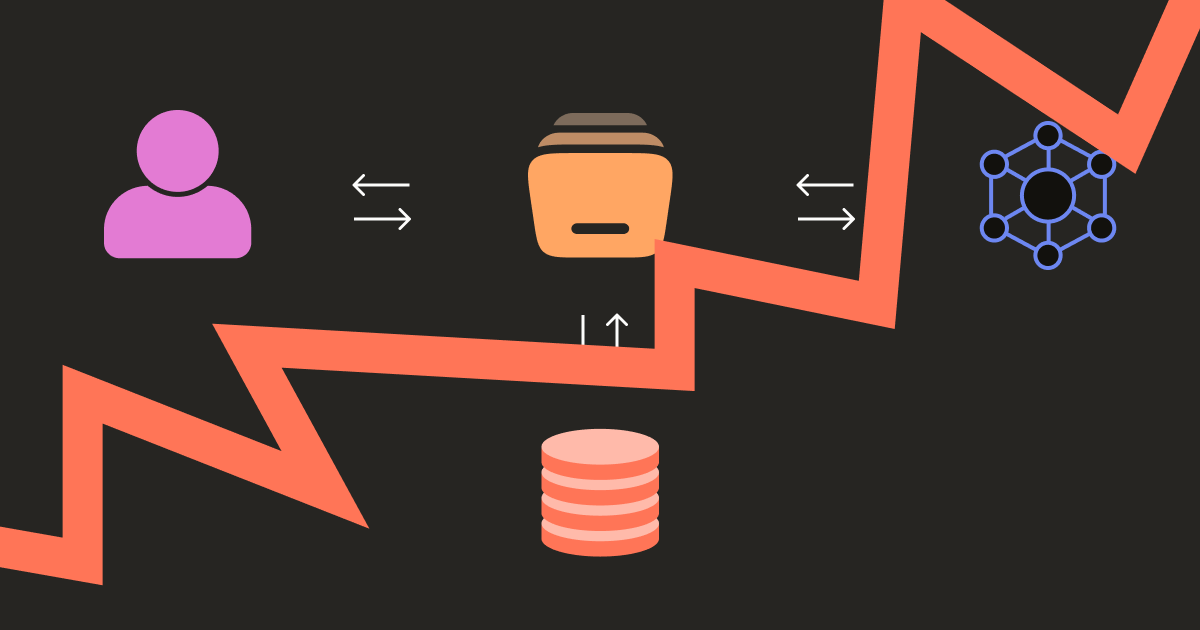
\includegraphics[width=0.9\textwidth]{images/presentacion/errors.png}
\end{columns}

\end{frame}

% -----------------------------------------------------

\begin{frame}{RAG no es verificación}

Si el documento contiene error:

\begin{itemize}
    \item \textbf{El modelo lo amplifica}.
    \item \textbf{No detecta contradicciones internas}.
    \item \textbf{No valida consistencia factual}.
\end{itemize}

RAG mejora acceso, no garantiza verdad.

\end{frame}

% =====================================================
\section{Evaluación}
\frame{\sectionpage}

\begin{frame}{Métricas de retrieval}
\begin{columns}[T]
\column{0.5\textwidth}
\begin{itemize}
    \item Precision@k
    \item Recall@k
    \item Mean Reciprocal Rank (MRR)
    \item nDCG
\end{itemize}

Sin evaluar retrieval, no se puede optimizar el sistema.
\column{0.5\textwidth}
\centering
 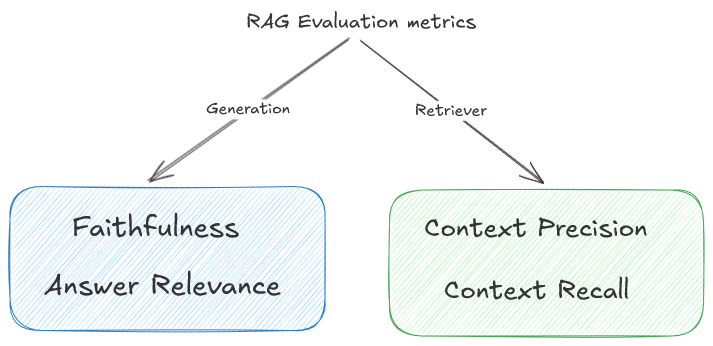
\includegraphics[width=0.9\textwidth]{images/presentacion/rag3.png}
\end{columns}
\end{frame}

% -----------------------------------------------------

\begin{frame}{Evaluación end-to-end}

Se debe medir:

\begin{itemize}
    \item \textbf{Coherencia final}.
    \item \textbf{Consistencia con fuente}.
    \item \textbf{Estabilidad entre ejecuciones}.
    \item \textbf{Trazabilidad} (citar fragmentos).
\end{itemize}

RAG sin trazabilidad es \textbf{opaco} y sin estabilidad \textbf{no es confiable}.

\end{frame}

% =====================================================
\section{Conclusiones}
\frame{\sectionpage}

\begin{frame}{RAG vs Fine-tuning}
En datos dinámicos, RAG suele ser preferible. \\
\vspace{2em}
\centering
\begin{tabular}{ll}
\toprule
\textbf{Fine-tuning} & \textbf{RAG} \\
\midrule
Cambia parámetros & No cambia parámetros \\
Integra conocimiento & Consulta conocimiento \\
Coste alto inicial & Coste por consulta \\
Riesgo de olvido & Modelo intacto \\
\bottomrule
\end{tabular}

\end{frame}

% -----------------------------------------------------

\begin{frame}{Lecciones aprendidas}
Es una arquitectura de \textbf{acceso a información}, no un mecanismo de aprendizaje.
\vspace{1.5em}
\begin{itemize}
    \item RAG no hace al modelo más inteligente.
    \item El sistema se especializa en un contexto.
    \item Incrementa el tamaño del prompt.
    \item Afecta al número de tokens utilizados.
\end{itemize}
\vspace{1.5em}
\textbf{Siguiente paso:} arquitecturas agénticas.
\end{frame}

\end{document}
